%Compile with PDFLaTeX
\documentclass[a4paper,10pt,english]{article}
\usepackage{mathptmx}
\renewcommand{\familydefault}{\rmdefault}
\usepackage{graphicx}
\usepackage{babel}
\usepackage{caption}
\usepackage{subcaption}
\usepackage{floatrow}
\usepackage{orstylet}
\makeatother
\begin{document}
\renewcommand{\figurename}{Fig.} 


\title{DRELL-YAN PROCESS BACKGROUND ESTIMATION USING\\ THE FAKE RATE METHOD}


\author{\uline{Marijus Ambrozas}, Andrius Juodagalvis}

\maketitle

\address{Institute of Theoretical Physics and Astronomy, Faculty of Physics, Vilnius University, Lithuania}

\rightaddress{marijus.ambrozas@ff.stud.vu.lt}

The Large Hadron Collider (LHC) at CERN produces high energy proton-proton collisions which allow us to
peek into the smallest building blocks of the Universe.
Protons in the collider can be seen as streams of quarks and gluons, according to the parton model.
Many different parton-parton interactions are possible during the proton collision.
Probabilities of different outcomes depend on the parton distribution functions (PDFs), which describe
the inner structure of the proton.
Precise knowledge of the PDFs is required for realistic estimation of the probabilities of very rare events.

The Drell-Yan process is a quark-antiquark annihilation resulting in a lepton-antilepton pair \cite{DY}.
High-precision measurements of the differential Drell-Yan cross section are useful for constraining the PDFs, as
well as for testing the perturbative framework of the Standard Model \cite{DY13}.
They are also important for many other experimental measurements where the Drell-Yan process
is a significant background \cite{Higgs, Zprime, SUSY}.

Lepton tracks that emerge from the Drell-Yan process are ususally well separated from any other particle tracks
produced in the event.
They are called ``isolated leptons.''
Several other processes can also lead to production of the isolated lepton pairs (for example, the
leptonic decay of a top quark-antiquark pair).
These processes can be easily confused with the Drell-Yan process and are referred to as backgrounds.
However, non Drell-Yan production of the isolated lepton pairs is not the only possible background.

A quark or a gluon may also be produced in the proton-proton collision.
Due to the confinement, it undergoes the hadronization process which results in a cone-shaped hadron stream, called a jet.
Heavy flavor jets (for example, bottom or charm jets) may contain an energetic lepton.
On very rare cases, some hadrons from a jet may reach muon detectors, which are located on the outermost
layers of modern particle detectors, and be confused with muons.
Ideally, in both of these cases the lepton track should not be isolated (it should be surrounded by a stream of hadrons).
Though, it is still  possible for the event reconstruction algorithm to misidentify a jet as an isolated lepton.
Therefore, jet events also contribute to the Drell-Yan backgrounds.

It is very difficult to predict the ammount of jet backgrounds from the simulation, because jet events have a very
large cross section and a very low probability to be misidentified as isolated lepton events.
Data-driven methods are used to estimate these kind of backgrounds.
The fake rate method is one of them.
This method relies on estimating the probability for a jet to be misidentified.
The estimated probability is then used to predict the ammount of jet events in experimental data.
The fake rate method and its use with the 2016 CERN CMS proton-proton collision data will be discussed in the presentation

The work is performed in collaboration with scientists from Seoul National University and University of Nebraska Lincoln.
Collaboration with CERN CMS experiment is supported by Lithuanian academy of sciences.
 
\vspace{-0.3cm}
\begin{figure}[H]
	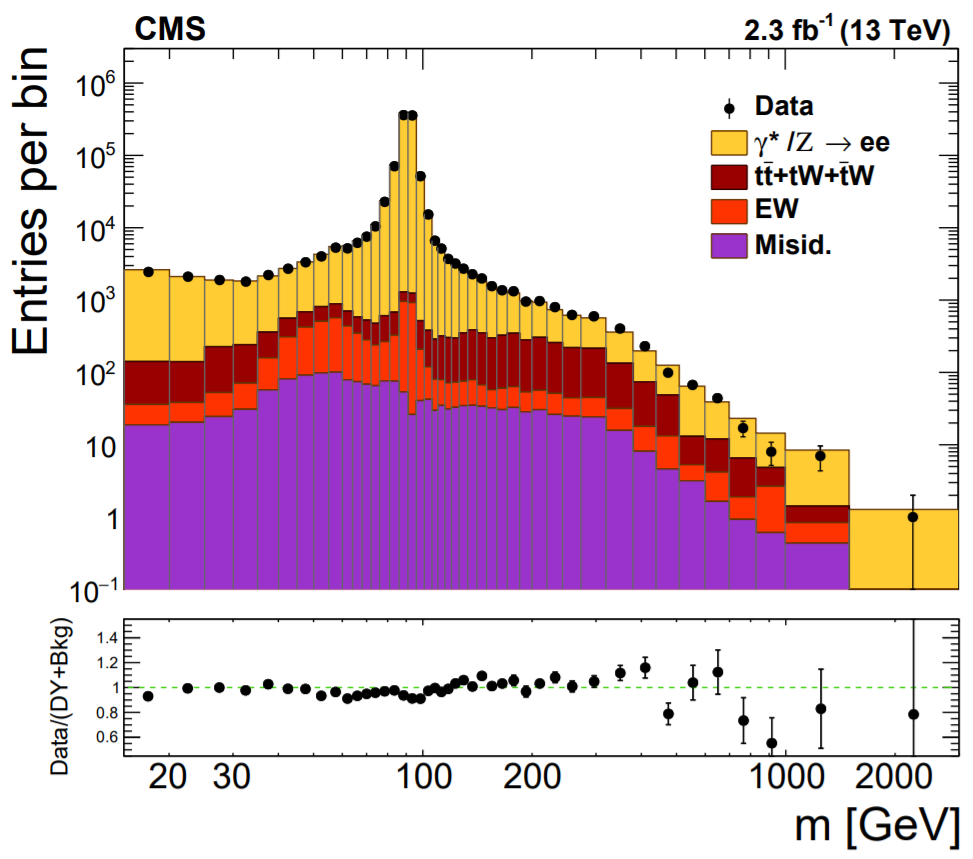
\includegraphics[width=.4\linewidth]{Figure1.png}
	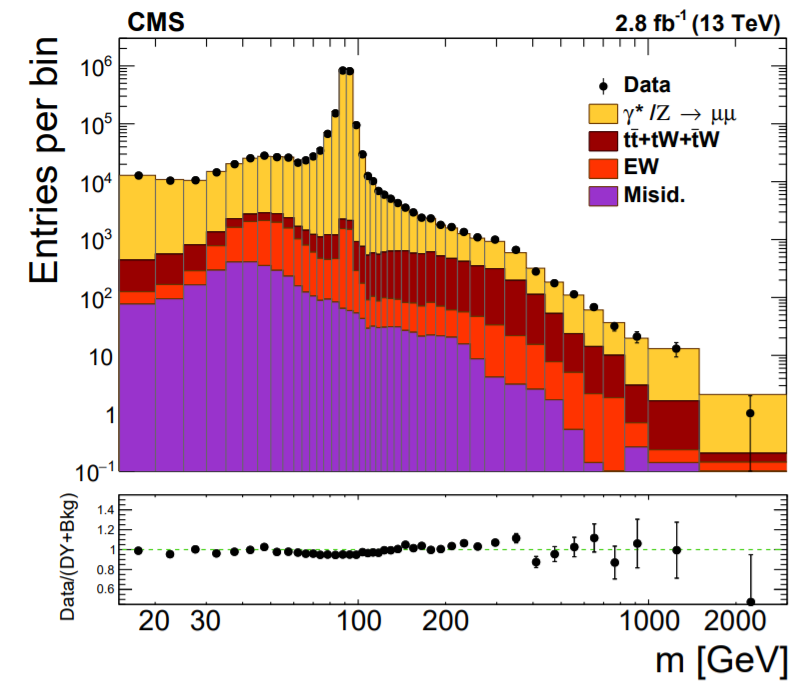
\includegraphics[width=.4\linewidth]{Figure2.png}
\vspace{-0.2cm}
\caption{Dielectron (left) and dimuon (right) invariant mass distributions in 2015 CMS data \cite{DY13}.
      Black dots represent the number of events measured with the CMS detector.
      Colored bars represent contribution of different processes.
      Yellow color marks the signal, i.e.\ the Drell-Yan process.
      ``EW'' denotes electroweak backgrounds.
      ``Misid.'' marks the contribution from misidentified jet events, estimated using the fake rate method.}
\end{figure}

\vspace{-0.5cm}
\begin{thebibliography}{References}
\bibitem{DY}S.\ D.\ Drell, T.\ M.\ Yan, Massive Lepton Pair Production in Hadron-Hadron Collisions at High-Energies,
Phys.\ Rev.\ Lett.\ \textbf{25}, 316 (1970).

\bibitem{DY13}CMS Collaboration, Measurement of the differential Drell-Yan cross section in proton-proton collisions
at $\sqrt{s}=13$ TeV, JHEP \textbf{12} 059 (2019).

\bibitem{Higgs}CMS Collaboration. Observation of the Higgs boson decay to a pair of tau leptons with the CMS detector.
Phys.\ Lett.\ B \textbf{779}, 283 (2018).

\bibitem{Zprime}CMS Collaboration. Search for high-mass resonances in dilepton final states in proton-proton collisions
at $\sqrt{s}=13$ TeV. JHEP \textbf{06} 120 (2018).

\bibitem{SUSY}CMS Collaboration. Search for supersymmetric partners of electrons and muons in proton-proton collisions
at $\sqrt{s}=13$ TeV. Phys.\ Lett.\ B \textbf{790} 005 (2019).
\end{thebibliography}

\end{document}
